\section{Experiments}
\label{sec:exp}

We evaluate our model extrinsically on classification tasks,
followed by intrinsic topic coherence.

\subsection{Classification with Topic Posteriors}
\label{subsec:exp_class}

%\begin{table}[t]
%  \centering
%  \small
%  \begin{threeparttable}
%  \begin{tabular}{lrrrr}
%    Method & \en-\intra & \si/\zh-\intra & \en-\cross & \si/\zh-\cross \\ \hline \hline
%    \multicolumn{5}{c}{Disaster Response} \\ \hline
%    \mcta\tnote{\dag} & 12.99 & 26.53 & 4.08 & 15.58 \\
%    \mtanchor\tnote{\dag} & 20.78 & 32.65 & 24.49 & 24.68 \\
%    \lda & 27.78 & 24.01 & 22.86 & 21.05 \\
%    \ptlda & 12.77 & 18.18 & 16.01 & 15.09 \\ \hline
%    \mtm & \textbf{42.86} & 23.08 & 22.22 & 26.67 \\
%    \mtm + \toplink & \textbf{42.86} & 23.08 & \textbf{35.29} & \textbf{33.33} \\
%    \mtm + \tfidf & 26.67 & \textbf{38.10} & 14.46 & 15.09 \\
%    \mtm + \tfidf + \toplink & 26.67 & \textbf{38.10} & 14.46 & 11.43 \\ \hline \hline
%    \multicolumn{5}{c}{Wikipedia} \\ \hline
%    \mcta\tnote{\dag} & 51.56 & 33.35 & 23.24 & 39.79 \\
%    \mtanchor\tnote{\dag} & 80.71 & 75.33 & 57.62 & 54.54 \\
%    \lda & 92.08 & 83.37 & 16.52 & 10.46 \\
%    \ptlda & 91.58 & 83.33 & 2.85 & 21.02 \\ \hline
%    \mtm & 92.98 & \textbf{86.48} & 74.69 & 64.48 \\
%    \mtm + \toplink & 92.98 & \textbf{86.48} & \textbf{78.13} & \textbf{83.08} \\
%    \mtm + \tfidf & \textbf{94.07} & 85.59 & 57.27 & 55.06 \\
%    \mtm + \tfidf + \toplink & \textbf{94.07} & 85.59 & 63.20 & 59.64 \\ \hline \hline
%  \end{tabular}
%  \caption{Our \mtm outperforms all the baselines in intra- and cross-lingual evaluations in F1 scores.}\label{tab:class}
%  \begin{tablenotes}
%    \item[\dag] Reported by~\newcite{yuan-2018-mtanchor}.  \jbgcomment{Would be good to have error bars on these if possible (can we also try a bar chart?)}
%  \end{tablenotes}
%  \end{threeparttable}
%\end{table}

\begin{figure}[t]
  \centering
  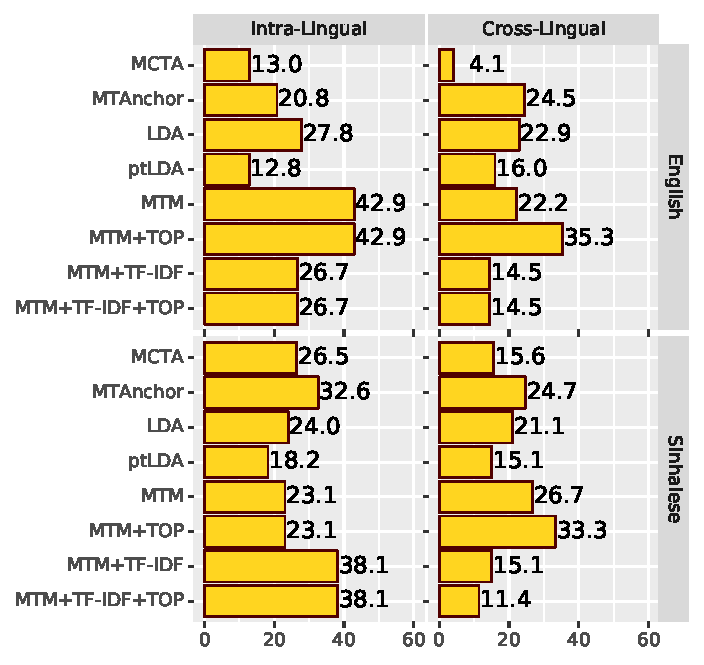
\includegraphics[width=\linewidth]{2019_emnlp_mtm/auto_fig/lorelei.pdf}
  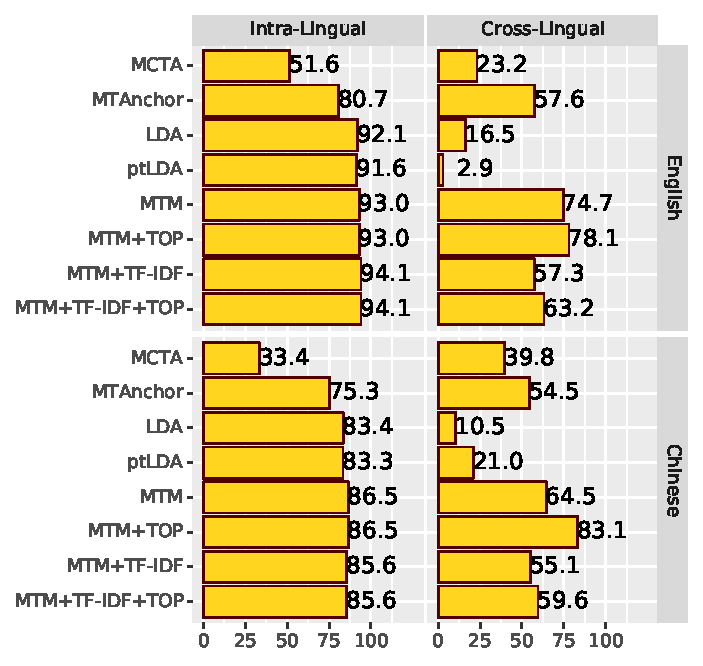
\includegraphics[width=\linewidth]{2019_emnlp_mtm/auto_fig/wiki.pdf}
  \caption{The F1 scores on disaster response (upper) and Wikipedia (lower) datasets. Our \mtm outperforms all the baselines in intra- and cross-lingual evaluations.\wycomment{It's hard to obtain the error bars. The datasets are just split into a training set and a test set, not cross-validation.}}\label{fig:f1}
\end{figure}

\jbgcomment{It seems that we never explicitly define the features.
  Did that get deleted?  Let's make sure that's explained at least at
  a high level here. \wycomment{We just never explicitly define them. I added it in the second paragraph.}}

We use two datasets for classification: Wikipedia documents in English (\en)
 and Chinese (\zh)~\cite{yuan-2018-mtanchor} and an
English-Sinhalese (\si) disaster response
dataset~\cite{strassel-2016-lorelei}.\footnote{More dataset details in
  the Supplement.}
%
Each dataset provides labeled documents and a
dictionary. \newcite{yuan-2018-mtanchor} extract the \en-\zh
dictionary from \textsc{mdbg}, while~\newcite{strassel-2016-lorelei}
construct the \en-\si dictionary from online resources and manual
annotation.\footnote{\textsc{mdbg}:
  \url{https://www.mdbg.net/chinese/dictionary?page=cc-cedict}}
%
Each Wikipedia document is labeled with one of the topics of
\emph{film}, \emph{music}, \emph{animals}, \emph{politics},
\emph{religion}, and \emph{food}. A portion of the disaster response
documents are labeled with one of eight types of needed rescue
resources: \emph{evacuation}, \emph{food supply},
\emph{search/rescue}, \emph{utilities}, \emph{infrastructure},
\emph{medical assistance}, \emph{shelter}, and \emph{water supply}.

We follow~\newcite{yuan-2018-mtanchor} for preprocessing (such as lemmatization for English and segmentation for Chinese) and use a linear \textsc{svm}
for classification.
%
For the Wikipedia dataset, we
report micro-F1 scores on a six-way classification.
 For the disaster response dataset, our goal is binary classification of
the need for \emph{evacuation} versus other assistance.
The classification uses features of topic posteriors: $\prob{k}{d} \equiv N_{d,k} / N_{d}$ which is the proportion of the tokens assigned to topic~$k$ in document~$d$.

The baselines include polylingual tree
\lda~\cite[\ptlda]{Hu-2014-ptlda} which encodes the dictionary as a
tree prior~\cite{andrzejewski-2009-dir-forest}, Multilingual Topic
Anchoring~\cite[\mtanchor]{yuan-2018-mtanchor}, and Multilingual
Cultural-common Topic Analysis~\cite[\mcta]{shi-2016-mtm-common}. We
also include \lda, which runs monolingually in each language. We use
20 topics and set hyper-parameters $\alpha=0.1$ and $\beta=0.01$
(if applicable).

Our evaluations are both intra- and cross-lingual. The intra-lingual
evaluation trains and tests classifiers on the same
language, while the cross-lingual evaluation trains
classifiers on one language and tests on another. In cross-lingual
evaluations, \mtanchor, \mcta, and \ptlda align topic spaces, so topic
posterior transformation is not necessary. \lda cannot transform topic
spaces, so we do not apply any transformation. For our \mtm, we
explore two transformation methods with~$\bm{\rho}$. The first
multiplies~$\bm{\rho}$ with a language's document topic distributions,
i.e.,
$\bm{\rho_{\text{\zh}\rightarrow \text{\en}}}
\bm{\theta_{\text{\zh}}}$ and vice versa. The second (\toplink),
transfers each document topic's probability mass to the topic in the
other language with the highest link weight.\footnote{An example of \toplink is available in the Supplement.}

Our \mtm has higher F1 both intra- and cross-lingually
(Figure~\ref{fig:f1}).\ignore{\footnote{\mtanchor and \mcta results
    are reported by~\newcite{yuan-2018-mtanchor}.}} \tfidf weighting
on translation pairs sometimes improves the intra-lingual F1,
although it hurts the cross-lingual F1. Connecting the top
linked topics (\toplink) is better than directly using the topic link
weight matrices. This indicates that~$\bm{\rho}$'s values have
some noise.

\jbgcomment{There should be a clearer transition here that says that
  the topics are aligned across languages; let's see if they make
  sense.\wycomment{Done.}}

\subsection{Looking at Learned Topics}
\label{subsec:exp_example}

\psrnewcomment{I've updated the subsection heading to make it clearer that this is example/analysis, not evaluation}

%\begin{table*}[t!]
%  \centering
%  \small
%  \begin{tabular}{lll}
%    Model & Language & Words \\ \hline \hline
%    \multirow{3}{*}{\mcta} & \zh & \multirow{3}{*}{
%        \begin{tabular}{lllllll}
%            \ch{主演} & \ch{改编} & \ch{本} & \ch{小说} & \ch{拍摄} & \ch{角色} & \ch{战士} \\
%            starring & adapt & this & novel & shoot & role & fighter \\
%            dog & san & movie & mexican & figher & novel & california
%        \end{tabular}} \\
%     & \zh-\tr & \\ \cline{2-3}
%     & \en & \\ \hline
%    \multirow{3}{*}{\mtanchor} & \zh & \multirow{3}{*}{
%        \begin{tabular}{lllllll}
%            \ch{主演} & \ch{改编} & \ch{饰演} & \ch{本片} & \ch{演员} & \ch{编剧} & \ch{讲述} \\
%            starring & adapt & act & this movie & actor & playwright & narrate \\
%            kong & hong & movie & official & martial & box & reception
%        \end{tabular}} \\
%     & \zh-\tr & \\ \cline{2-3}
%     & \en & \\ \hline
%    \multirow{3}{*}{\lda} & \zh & \multirow{3}{*}{
%        \begin{tabular}{lllllll}
%            \ch{电影} & \ch{部} & \ch{美国} & \ch{上映} & \ch{英语} & \ch{剧情} & \ch{片} \\
%            movie & movie quantifier & USA & release & English & plot & movie \\
%            film & star & direct & release & action & plot & character
%        \end{tabular}} \\
%     & \zh-\tr & \\ \cline{2-3}
%     & \en & \\ \hline
%    \multirow{3}{*}{\ptlda} & \zh & \multirow{3}{*}{
%        \begin{tabular}{lllllll}
%            \ch{电影} & \ch{胶片} & \ch{星} & \ch{动作} & \ch{释放} & \ch{影片} & \ch{剧情} \\
%            movie & film & star & action & release & movie & plot \\
%            film & star & direct & action & release & plot & write
%        \end{tabular}} \\
%     & \zh-\tr & \\ \cline{2-3}
%     & \en & \\ \hline
%    \multirow{5}{*}{\mtm} & \zh & \multirow{5}{*}{
%        \begin{tabular}{lllllll}
%            \ch{电影} & \ch{部} & \ch{上映} & \ch{动画} & \ch{故事} & \ch{作品} & \ch{英语} \\
%            movie & movie quantifier & release & animation & story & works & English \\
%            film & direct & star & release & action & plot & production \\
%            kill & find & death & attack & escape & return & back \\
%            shrine & japanese & temple & japan & shinto & kami & god
%        \end{tabular}} \\
%     & \zh-\tr & \\ \cline{2-3}
%     & \en-1 (0.20) & \\
%     & \en-2 (0.12) & \\
%     & \en-3 (0.11) & \\ \hline
%    \multirow{5}{*}{\tabincell{l}{\mtm +\\ \tfidf}} & \zh & \multirow{5}{*}{
%        \begin{tabular}{lllllll}
%            \ch{电影} & \ch{部} & \ch{上映} & \ch{美国} & \ch{英语} & \ch{导演} & \ch{片} \\
%            movie & movie quantifier & release & USA & English & director & movie \\
%            film & direct & star & action & release & plot & movie \\
%            film & kill & find & escape & attack & return & back \\
%            character & series & star & game & trek & create & episode
%        \end{tabular}} \\
%     & \zh-\tr & \\ \cline{2-3}
%     & \en-1 (0.32) & \\
%     & \en-2 (0.24) & \\
%     & \en-3 (0.09) & \\ \hline
%  \end{tabular}
%  \caption{The topics of \underline{Movies} given by models. \zh-\tr indicates the English translations of the Chinese words. For the Chinese topics given by our \mtm, the top three English topics and their link weights are also given.}\label{tab:example}
%\end{table*}

\begin{table}[t!]
  \centering
  \small
  \begin{tabular}{ll}
    Lang. & Words \\ \hline \hline
    \multicolumn{2}{c}{\mcta} \\ \hline
    \multirow{2}{*}{\zh} & \ch{主演} (starring), \ch{改编} (adapt), \ch{本} (this), \\
     & \ch{小说} (novel), \ch{拍摄} (shoot), \ch{角色} (role) \\
    \en & dog, san, movie, mexican, fighter, novel \\ \hline \hline
    \multicolumn{2}{c}{\mtanchor} \\ \hline
    \multirow{2}{*}{\zh} & \ch{主演} (starring), \ch{改编} (adapt), \ch{饰演} (act), \\
     & \ch{本片} (the movie), \ch{演员} (actor), \ch{编剧} (playwright) \\
    \en & kong, hong, movie, official, martial, box \\ \hline \hline
    \multicolumn{2}{c}{\lda} \\ \hline
    \multirow{2}{*}{\zh} & \ch{电影} (movie), \ch{部} ([Q] movie),\footnote{In Tables~\ref{tab:example} and~\ref{tab:topic_links}, ``[Q]'' denotes the Chinese word is a counter for the following English word.} \ch{美国} (USA), \\
     & \ch{上映} (release), \ch{英语} (English), \ch{剧情} (plot) \\
    \en & film, star, direct, release, action, plot \\ \hline \hline
    \multicolumn{2}{c}{\ptlda} \\ \hline
    \multirow{2}{*}{\zh} & \ch{电影} (movie), \ch{胶片} (film), \ch{星} (star), \\
     & \ch{动作} (action), \ch{释放} (release), \ch{影片} (movie) \\
    \en & film, star, direct, action, release, plot \\ \hline \hline
    \multicolumn{2}{c}{\mtm} \\ \hline
    \multirow{2}{*}{\zh} & \ch{电影} (movie), \ch{部} ([Q] movie), \ch{上映} (release),  \\
     & \ch{动画} (animation), \ch{故事} (story), \ch{作品} (works),  \\
    \en (.20) & film, direct, star, release, action, plot \\
    \en (.12) & kill, find, death, attack, escape, return \\
    \en (.11) & shrine, japanese, temple, japan, shinto, kami \\ \hline \hline
    \multicolumn{2}{c}{\mtm + \tfidf} \\ \hline
    \multirow{2}{*}{\zh} & \ch{电影} (movie), \ch{部} ([Q] movie), \ch{上映} (release),  \\
     & \ch{美国} (USA), \ch{英语} (English), \ch{导演} (director) \\
    \en (.32) & film, direct, star, action, release, plot \\
    \en (.24) & film, kill, find, escape, attack, return \\
    \en (.09) & character, series, star, game, trek, create \\ \hline \hline
  \end{tabular}
  \caption{The \underline{Movies} topics given by models. For the Chinese (\zh) topics given by \mtm, the top three English (\en) topics and their link weights are also given.\wycomment{I cut the number of top words from 7 to 6 to save space as the last word does not affect the evaluation much.}}\label{tab:example}
\end{table}

Past \mtms align topics across languages but our \mtm does not, so we compare the topics across models to see how they differ.
We look at the \underline{Movies} topics from the Wikipedia dataset (Table~\ref{tab:example}). For the Chinese \mtm topics, we show the three English topics with the highest link weights.

The topics are about \underline{Movies}, but the \mcta and \mtanchor
topics do not rank ``movie'' or ``\ch{电影} (\pinyin{dian4}
\pinyin{ying3})'' at the top.
%
The \ptlda topics, although aligned
well, incorrectly align\jbgcomment{``problems'' is vague, be specific\wycomment{Done.}} some Chinese words. ``\ch{胶片}
(\pinyin{jiao1} \pinyin{pian4})'' means ``\emph{photographic}
film'',\ignore{instead of ``movie''} while ``\ch{释放}
(\pinyin{shi4} \pinyin{fang4})'' means \emph{release} as in ``let something go'', not movie distribution.
%
\ptlda links words based on translations without looking at the
context, which causes problems with multiple-sense words.
%
The \lda and \mtm topics are generally coherent.

\psrnewcomment{I am shifting the emphasis in this paragraph to be more
  about the topics, since the topic \emph{links} are the focus of the
  next subsection.}

The \mtm's unique joint modeling of weighted topic links also recovers
additional topical structure: after linking respective \en-\zh
\underline{Movies} topics,\jbgcomment{It's unclear what ``we
  find'' means here; let's tighten up wording\wycomment{Done.}} the next linked topics are
\underline{Action Movies} (``kill'', ``death'', ``attack'', and
``escape'').
%
Further, the models capture a degree of connection between
\underline{Movies} and \underline{Computer Games} (\mtm + \tfidf) and
\underline{Japanese Animations} (\mtm).
%
\psrnewcomment{Is ``unique joint modeling'' accurate? I'm trying to
  focus here on the jointness of the model producing the topics rather
  than the links, which are in the next subsection. Also, I'm kind of
  on the fence on saying anything about the 3rd-ranked links. We're
  trying to put a positive spin on it, but I could also see these
  being interpreted as stretching it a little to far or just
  incorrect. Either way, we're kind of begging the question of how far
  down the link-weights list you set your cutoff of what's relevant or
  not. One could possibly hedge this by adding the word ``arguably'',
  to say ``Further the models arguably capture a degree of...'' so at
  least it's clear we know we're stretching it a little
  bit. \wycomment{I think the phrasing and to focus on the joint
    modeling are good. I added more info to address its uniqueness.}}


\subsection{Looking at Learned Topic Links}
\label{subsec:exp_topic_link}

\psrnewcomment{I've updated the subsection heading to make it clearer that this is example/analysis, not evaluation}

%\begin{table*}[t!]
%  \centering
%  \small
%  \begin{tabular}{lrl}
%    Language & Weight & Words \\ \hline \hline
%    \zh-0 & -- & \multirow{4}{*}{
%        \begin{tabular}{lllllll}
%            \ch{学名} & \ch{它们} & \ch{呈} & \ch{白色} & \ch{长} & \ch{黑色} & \ch{厘米} \\
%            scientific name & they & show & white & long & black & centimeter \\
%            specie & bird & eagle & genus & white & owl & black\\
%            breed & chicken & white & goose & bird & black & list
%        \end{tabular}} \\
%    \zh-0-\tr & -- &  \\
%    \en-12 & 0.57 &  \\
%    \en-19 & 0.13 &  \\ \hline
%    \zh-14 & -- & \multirow{4}{*}{
%        \begin{tabular}{lllllll}
%            \ch{主义} & \ch{组织} & \ch{美国} & \ch{革命} & \ch{运动} & \ch{政府} & \ch{人民} \\
%            -ism & organization & USA & evolution & campaign & government & people \\
%            sex & law & act & sexual & marriage & court & legal \\
%            traffic & victim & government & trafficking & child & force & country
%        \end{tabular}} \\
%    \zh-14-\tr & -- & \\
%    \en-16 & 0.32 & \\
%    \en11 & 0.17 & \\ \hline
%%    \en-1 & -- & \multirow{5}{*}{
%%        \begin{tabular}{lllllll}
%%            abortion & government & report & muslim & death & arrest & iran \\
%%            \ch{伊斯兰} & \ch{穆斯林} & \ch{伊斯兰教} & \ch{阿拉伯语} & \ch{阿拉伯} & \ch{世纪} & \ch{帝国} \\
%%            Islam & muslim & Islam & Arabic & Arab & century & empire \\
%%            \ch{主义} & \ch{社会} & \ch{历史} & \ch{文化} & \ch{发展} & \ch{研究} & \ch{哲学} \\
%%            -ism & society & history & culture & develop & research & philosophy
%%        \end{tabular}} \\
%%    \zh-15 & \multirow{2}{*}{0.16} & \\
%%    \zh-15-\tr & & \\
%%    \zh-4 & \multirow{2}{*}{0.13} & \\
%%    \zh-4-\tr & & \\ \hline
%    \en-10 & -- & \multirow{5}{*}{
%        \begin{tabular}{lllllll}
%            album & release & record & music & song & single & feature \\
%            \ch{专辑} & \ch{张} & \ch{发行} & \ch{音乐} & \ch{首} & \ch{唱片} & \ch{歌手} \\
%            album & album quantifier & release & music & song quantifier & record & singer \\
%            \ch{音乐} & \ch{乐团} & \ch{艺术} & \ch{创作} & \ch{奖} & \ch{演出} & \ch{担任} \\
%            music & musical group & art & create & prize & perform & serve
%        \end{tabular}} \\
%    \zh-9 & \multirow{2}{*}{0.30} & \\
%    \zh-9-\tr & & \\
%    \zh-17 & \multirow{2}{*}{0.20} & \\
%    \zh-17-\tr & & \\ \hline
%  \end{tabular}
%  \caption{Topics are linked because they have overlap in topical words. Although explicit word translations can help identify related topics, our \mtm can also infer the topic relations beyond words, e.g., \zh-14 and \en-16.}\label{tab:topic_links}
%\end{table*}

\begin{table}[t!]
  \centering
  \small
  \begin{tabular}{ll}
    Lang. & Words \\ \hline \hline
    \multirow{2}{*}{\zh-0} & \ch{学名} (scientific name), \ch{它们} (they), \ch{呈} (show),  \\
     & \ch{白色} (white), \ch{长} (long), \ch{黑色} (black) \\
    \en-12 (.57) & specie, bird, eagle, genus, white, owl \\
    \en-19 (.13) & breed, chicken, white, goose, bird, black \\ \hline
    \multirow{3}{*}{\zh-14} & \ch{主义} (-ism), \ch{组织} (organization), \\
     & \ch{美国} (USA), \ch{革命} (revolution), \\
     & \ch{运动} (campaign), \ch{政府} (government)  \\
    \en-16 (.32) & sex, law, act, sexual, marriage, court \\
    \en-11 (.17) & traffic, victim, government, trafficking, child, force \\ \hline
    \en-10 & album, release, record, music, song, single \\
    \multirow{2}{*}{\zh-9 (.30)} & \ch{专辑} (album), \ch{张} ([Q] album), \ch{发行} (release), \\
     & \ch{音乐} (music), \ch{首} ([Q] song), \ch{唱片} (record) \\
    \multirow{2}{*}{\zh-17 (.20)} & \ch{音乐} (music), \ch{乐团} (musical group), \ch{艺术} (art), \\
     & \ch{创作} (create), \ch{奖} (award), \ch{演出} (perform) \\ \hline
  \end{tabular}
  \caption{Topics are linked because they have overlap in topical words. Our \mtm can also infer the topic relations beyond words, e.g., \zh-14 and \en-16.}\label{tab:topic_links}
\end{table}

We give more examples of weighted \mtm topic links in
Table~\ref{tab:topic_links}.
%
High-weighted \underline{Biology} (\zh-0, \en-12, and \en-19) and
\underline{Music} topics (\en-10, \zh-9, and \zh-17) are characterized
by cross-lingual words in common.
%
The model can also infer topic links beyond words, linking topics when
the topical words have few direct translations but are related in
senses.
%
For instance, \zh-14 is about the ``campaigns'' against
``government''.
%
Only ``government'' overlaps with \en-16 and \en-11, but \mtm
identifies the two English topics as the top linked topics for \zh-14:
\en-16 is about the ``campaign'' in \underline{Sexual Rights}, while
\en-11 is about the \underline{Crime} of human trafficking.
%
This shows that our \mtm can incorporate word translations and infer
more cross-lingual word and topic relationships.

%\subsection{Evaluating Topic Coherence on Less Comparable Corpora}
\subsection{Evaluating Topic Coherence}
\label{subsec:exp_pmi}

\psrnewcomment{I've updated the subsection heading to make it clearer
  that this is example/analysis, not evaluation. I've also shortened
  the subsection name so it fits on one line.}

\begin{figure}[t!]

\jbgcomment{It would be good to use ggplot2 or plot9 to create figures \wycomment{Done.} But the code is not in repo (figures.py).  Would be good to put caption on top and to make the font a little bigger.\wycomment{Code is added. I move the legend to the top and the figures are larger now.}}

\centering
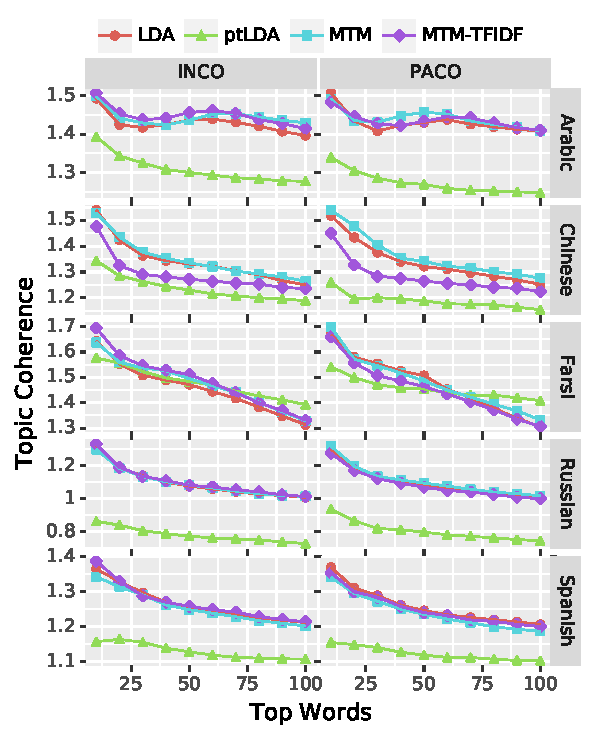
\includegraphics[width=\linewidth]{2019_emnlp_mtm/figures/cv_vertical.pdf}
\caption{Topic coherence on \inco and \paco datasets with the number of top words in each topic.}\label{fig:cv}
\end{figure}

We intrinsically evaluate models' topic coherence on two sets of
preprocessed bilingual Wikipedia corpora~\cite{hao-2018-mtm-doc-link}
that vary in ``nonparallelness''.
%
Both pair English with Arabic, Chinese, Spanish, Farsi, and Russian.
%Each bilingual corpus contains around 2,000 documents
% for both languages.
In \paco, 30\% of documents have direct translations across languages,
and in \inco none has direct translations. Dictionaries are extracted
fromn
Wiktionary.\footnote{\url{https://dumps.wikimedia.org/enwiktionary/}}
Standard preprocessing has already been applied to the datasets,
including stemming, stop word removal, and high-frequency word
removal.
%The first dataset is partially comparable
%(\paco)---30\% of the documents have direct translations in the other
%language. The second one is incomparable (\inco), i.e., no documents
%have direct translations.

\jbgcomment{if there's time, would be good to do posthoc links of LDA
  topics\wycomment{Sorry, this is difficult given my laptop's data loss and the space limit.}}

We use an intra-lingual metric to evaluate topic
coherence~\cite{lau-2014-auto-word-intrusion}: for every topic, we
compute its top~$N$ words' average pairwise \pmi score
on a disjoint subset of Wikipedia
documents~\cite{hao-2018-mtm-doc-link}. We report average
coherence with~$N$ from 10 to 100 with a step size of 10 (five-fold
cross-validation). We use the same translation pair weighting options
as in our classification tasks and also compare against monolingual \lda
and \ptlda~\cite{Hu-2014-ptlda}.

\mtm is no worse than \lda and sometimes slightly
better (Figure~\ref{fig:cv}). \tfidf weighting on translation pairs
sometimes further improves coherence (e.g., Arabic, Farsi,
Russian, and Spanish on \inco) but occasionally hurts (e.g.,
Chinese). \ptlda mostly works poorly, except on Farsi with a high number
of top words. \ptlda aligns topic spaces, which is hard for
low-comparability data, thus sacrificing coherence
for alignment; in contrast \mtm only connects topics when they align well in senses.

\subsection{Topic Coherence vs. Target Language Corpora Sizes}
\label{subsec:topic_link_exp_target_ratio}

\begin{figure}[t]
  \centering
  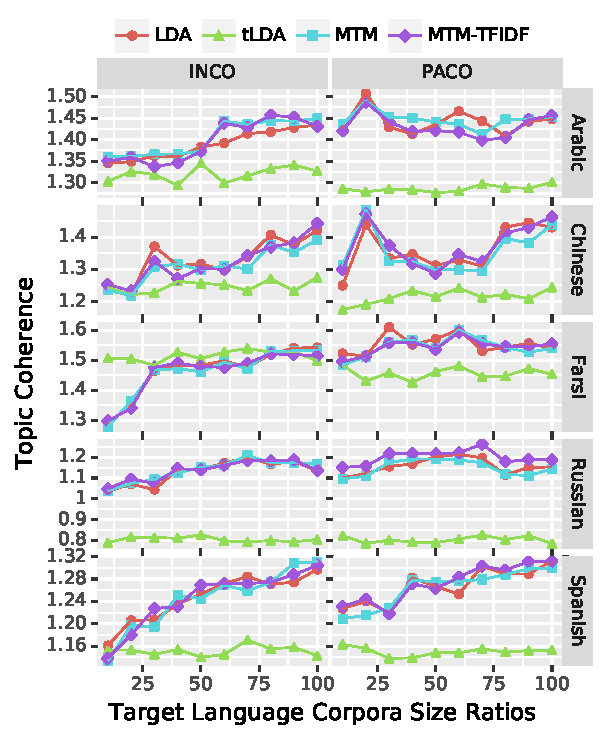
\includegraphics[width=\linewidth]{2019_emnlp_mtm/figures/ratio_vertical.pdf}
  \caption{The models' topic coherence on \inco and \paco datasets
    when the sizes of target language corpora grow from 10\% to 100\%,
    with a step size of 10\%.  \jbgcomment{``performance'' was here;
      make sure you're following style guidelines
      consistently.\wycomment{Done.}}}\label{fig:ratio}
\end{figure}

We next vary the size of target language (non-English languages in
\paco and \inco) corpora: how much can \mtm help topic coherence for
low-resource languages?
%
We start from 10\% of the randomly-selected documents in
target languages and incrementally add more target language documents
at a step size of 10\% until it reaches 100\%.
%
Meanwhile, we always use 100\% of the English documents.
%
We train monolingual \lda, \ptlda, and \mtms with and without \tfidf
weighting on translation pairs on each setting and evaluate the topic
coherence on the same reference corpora using the top thirty words of
each topic (Figure~\ref{fig:ratio}).

In most cases, the topic coherence improves with larger target corpora, except Arabic and Russian on \paco.
%
This confirms our intuition that more data yield a better topic model.
%
\mtm is helpful in cases when the target language corpora sizes are
small, e.g., Chinese and Russian with 10\% or 20\% of the corpora.
%
\tfidf weighting is not consistently better or worse
than equal weights.

The \ptlda with tree priors based on dictionaries performs poorly in
topic coherence, except Farsi in \inco.
%
In most cases, its topic coherence is substantially below others' and
improves little when the target corpora grow.

%\subsection{Target Language Corpus Size}
%\label{subsec:exp_target_ratio}
%
%The experiments are still running, so the results will be added if obtained in time.

%In this section, we study how the sizes of the secondary language corpora affect the topic coherence to simulate the situation when dealing with low-resource languages. In these experiments, we use all of the English documents and vary the size of the secondary language corpora. We randomly create the secondary language corpora by sampling from the original documents and start from 10\% to 100\%, with a step size of 10\%. Then we train a series of \mtms using the English documents and the sampled documents. We run each pair 5 times and report the average topic coherence scores.
%
%The topic coherence scores on the top 100 words given by \lda, \mtm, and \mtm with \tfidf weighting on both~\paco (Figure~\ref{fig:ratio_paco}) and~\inco (Figure~\ref{fig:ratio_inco}) datasets improve as the sizes of the secondary language corpora increase. \mtm, both with and without \tfidf weighting, works slightly better than \lda, although not significantly. \wycomment{Maybe compute the average over all sizes?} The \tlda's performance does not improve with the secondary language corpora sizes. Although it works the best on Farsi, its performance is a lot worse than other models on the rest of the languages.
%
%\begin{figure*}[t]
%\centering
%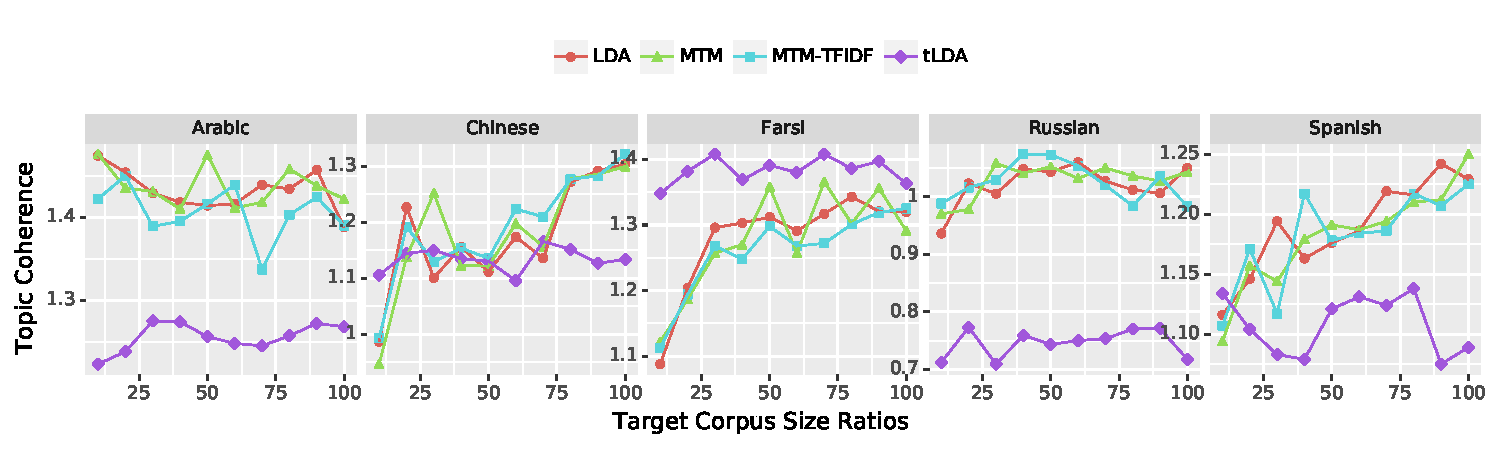
\includegraphics[width=\linewidth]{2019_emnlp_mtm/figures/paco_ratio.pdf}
%\caption{Various target corpus size results on \paco. \wycomment{TODO: Better caption.}}\label{fig:ratio_paco}
%\end{figure*}
%
%\begin{figure*}[t]
%\centering
%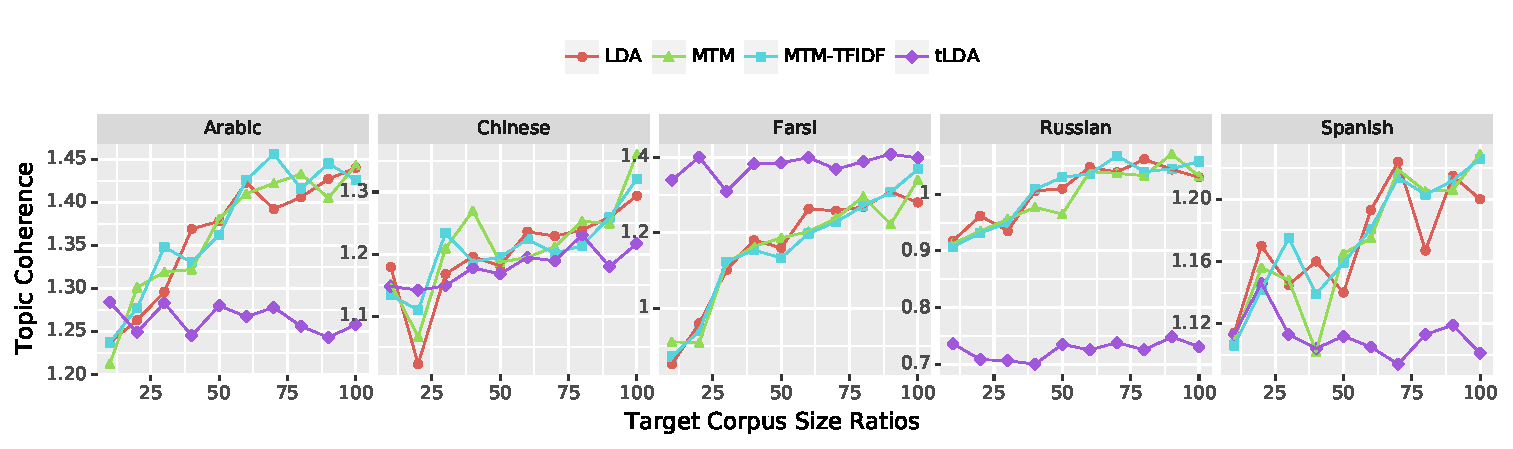
\includegraphics[width=\linewidth]{2019_emnlp_mtm/figures/inco_ratio.pdf}
%\caption{Various target corpus size results on \inco. \wycomment{TODO: Better caption.}}\label{fig:ratio_inco}
%\end{figure*}
